\documentclass{beamer}
%[aspectratio=169]   \usepackage[czech]{babel}
\usepackage{apo-lecture}
\usepackage{pdfpages}
\usepackage{pdfcomment}
\usepackage{listings}
\usepackage{array,multirow}

\subtitle{Lekce 07. Vstup a výstup}
\author{Pavel Píša \phantom{xxxxxxxxx} Petr Štěpán \\ \small\texttt{pisa@fel.cvut.cz}\phantom{xxxx}\small\texttt{stepan@fel.cvut.cz}}
\begin{document}

\maketitle

\section{Vstupy a výstupy}

\begin{frame}
\frametitle{Cíl dnešní přednášky}

\begin{itemize}
 \item Projít, jaké jsou možnosti vstupu a výstupu v počítači
 \item Periférie mapované do paměti
 \item Příklady v QtRvSim
 \item PCI a PCIe sběrnice
\end{itemize}
\end{frame}


\begin{frame}[shrink=10]
\frametitle{Architektura počítače -- John von Neumann}
\begin{center}
\includegraphics[width=0.5\textwidth]{cpu-vonNeumann.pdf}
\hfill
\includegraphics[width=0.15\textwidth]{fig/vonNeumann.png}
\end{center}
\begin{itemize}
\item 5 základních jednotek – řídicí jednotka, aritmeticko-logická jednotka, paměť, vstup (vstupní zařízení), výstup (výstupní zařízení)
\item Architektura počítače by neměla být závislá na řešené úloze, měla by umět provádět program uložený v paměti. Program řídí, co počítač vykonává za instrukce a tím jaké dostane výsledky.
\item Program a data jsou uložena ve stejné paměti, složené z buněk (jednotek) stejné velikosti. Oproti tomu Harvardská architektura měla jeden typ paměti pro program a jiný typ paměti pro data.
\item Další instrukce, která se bude vykonávat je uložena v následující buňce paměti (mimo skoků v programu)
\item Instrukce provádějí aritmetické a logické operace, přesuny dat z/do paměti, skoky a větvení programu a speciální řídicí instrukce.
\end{itemize}
\end{frame}

\begin{frame}
\frametitle{Návrh CPU z přednášky 5}
\includegraphics[width=0.95\textwidth]{cpu_design2.pdf}
\end{frame}

\begin{frame}
\frametitle{Propojení CPU s pamětí a perifériemi}
\begin{columns}
\begin{column}{0.4\textwidth}
\end{column}
\begin{column}{0.6\textwidth}  
\begin{itemize}
\item Adresová sběrnice (A0..A31) může být oddělená, nebo multiplexovaná, nebo sdílet stejné signály jako datová část
\item Datová sběrnice (D0..D31) může být obousměrná, nebo oddělená pro každý směr zvlášť, pralelní nebo sériová
\item Řídicí signály sběrnice
\item IOW, IOR se používají pokud jsou vstupní a výstupní periférie oddělené od paměti
\item BE0 to 3 -- pokud je povoleno čtení bajtů na sběrnici širší než 8 bitů.
\end{itemize}
\end{column}
\end{columns}
\end{frame}

\begin{frame}
\frametitle{Klasifikace periférií}
Chování:
\begin{itemize}
\item jenom vstup
\item jenom výstup
\item vstup i výstup (v současnosti většina zařízení)
\end{itemize}

Připojení:
\begin{itemize}
\item přímé propojení CPU a periférie
\item hierarchické -- propojení přes jiné periférie (bridge)
\end{itemize}

Partner:
\begin{itemize}
\item člověk -- jiné parametry komunikace
\item počítač -- většinou rychlejší komunikace
\item prostředí -- senzory a aktuátory
\end{itemize}

Parametry přenosu:
\begin{itemize}
\item kapacita přenosové linky -- maximální možnosti přenosu
\item latence -- čas, do kterého se zareaguje na přenos dat
\end{itemize}
\end{frame}

\begin{frame}
\frametitle{Klasifikace periférií}
Příklady periférií komunikujících s lidmy:
\begin{itemize}
\item klávesnice -- sice jen vstup, ale moderní často i výstup led diody, velmi malá přenosová rychlost, latence až do 200ms 
\item mikrofon/reproduktory -- přenosová rychlost až 8Mbit/s, latence záleží na aplikaci, pro komunikaci
\item tiskárny/scanery -- přenosová rychlost podle připojení, na latency nezáleží (v řádech vteřin)
\end{itemize}

Příklady periférií pro kounikaci mezi počítači
\begin{itemize}
\item modem -- 
\item sítě/WLAN -- 
\item datová úložistě -- HDD, SSD, magnetopáskové jednotky
\end{itemize}

Příklady senzorů a aktuátorů:
\begin{itemize}
\item kamera, laserové hloubkoměry
\item aktuátory -- motory DC/PMSM 
\end{itemize}
\end{frame}

\begin{frame}
\frametitle{Způsoby komunikace s periférií}
Data pouze na dotaz:
\begin{itemize}
\item zařízení čeká, až ho CPU osloví a zašle data na výstup, nebo požádá o připravená data ze vstupu
\item pomalejší komunikace, CPU musí aktivně zjišťovat, zda jsou připravená data k příjmu
\end{itemize}

Periférie využívá přerušení k signalizaci svého stavu:
\begin{itemize}
\item pokud dojde ke změně stavu, periférie vyvolá přerušení (přednáška 9)
\item CPU pak aktivně čte, nebo zapisuje data na periférii
\end{itemize}

Periférie využívá přímý přístup do paměti:
\begin{itemize}
\item využívá také přerušení
\item CPU nastaví pouze z/do jaké adresy v paměti se data budou číst/zapisovat a periférie sama řídí přenos dat
\item po ukončení periférie vyvolá přerušení a CPU zkontroluje výsledek přenosu (zda bylo vše v pořádku, nebo došlo k chybě)
\end{itemize}

\end{frame}

\begin{frame}
\frametitle{Zpracování periférií -- Linux (zjednodušeno)}
\begin{columns}
\begin{column}{0.4\textwidth}
Programy komunikují s perifériemy pomocí operačního systému a systémového volání a ovladačů periferií(přehled v přednášce 10, podrobně v předmětu OSY).

\bigskip
Další možností je komunikace přes sdílenou paměť -- náplň dnešní přednášky.
\end{column}
\begin{column}{0.58\textwidth}  
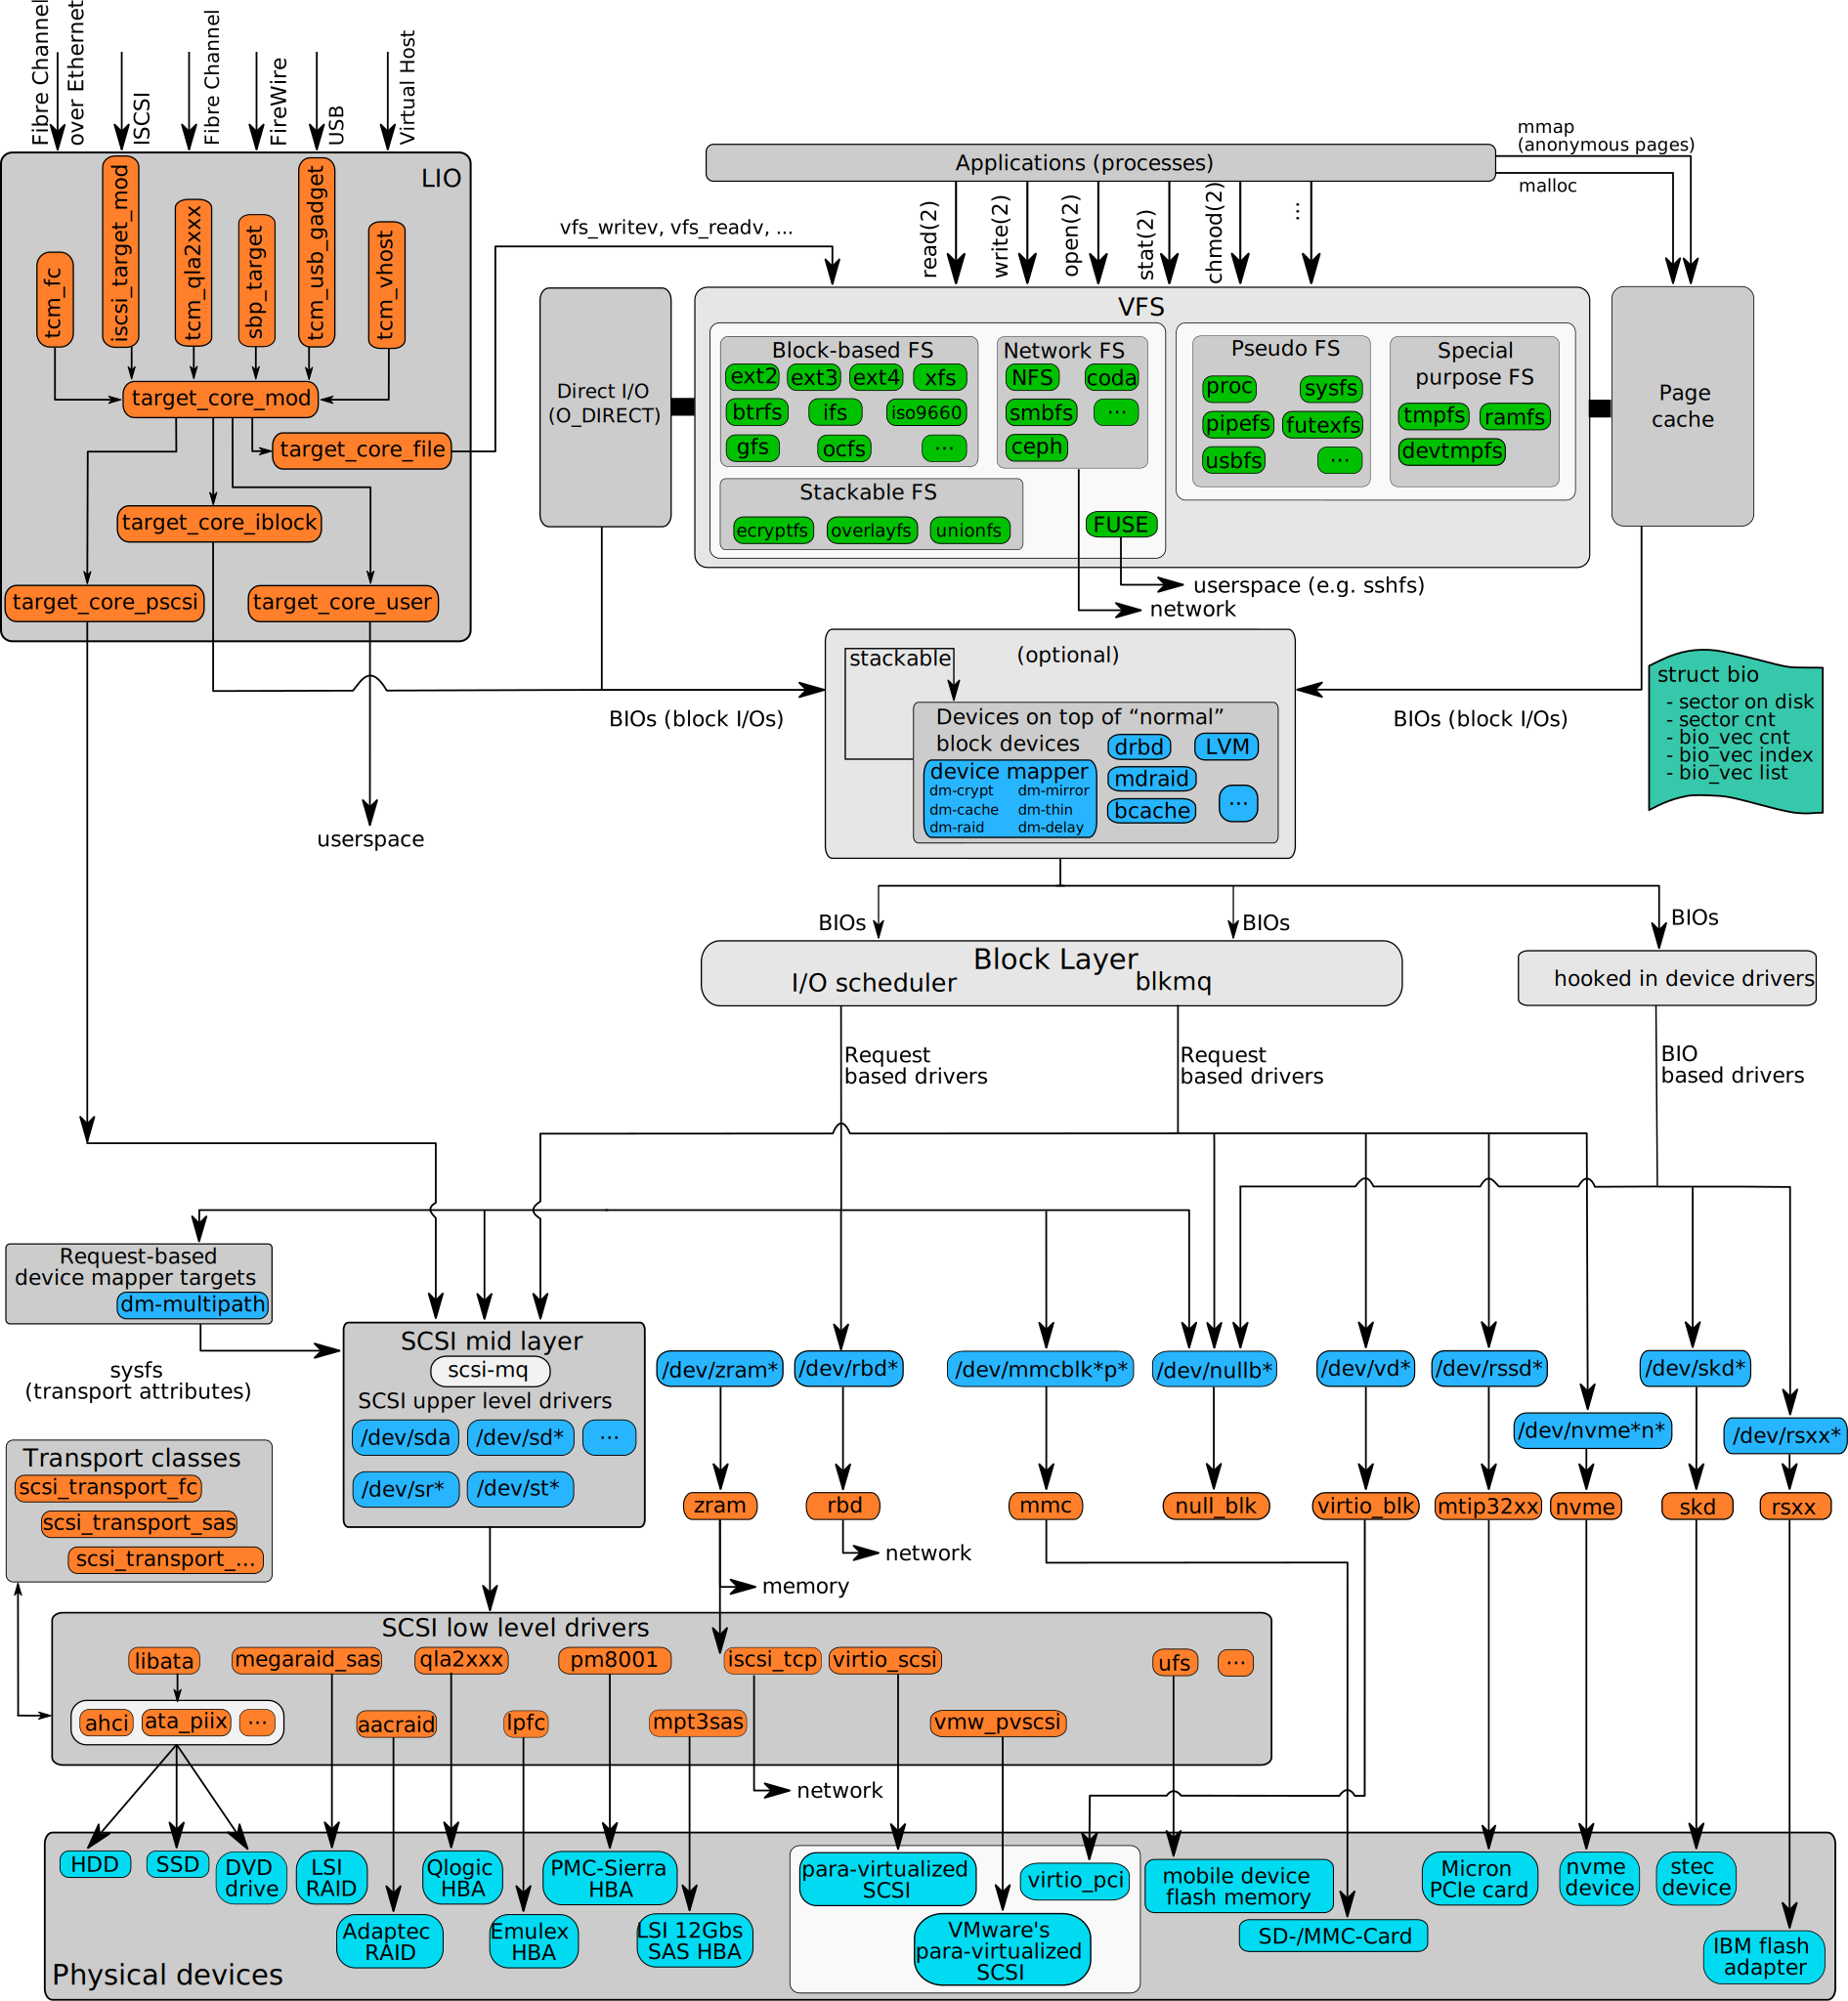
\includegraphics[width=\textwidth]{linux.pdf}
\end{column}
\end{columns}
\end{frame}


\begin{frame}
\frametitle{Systémová volání}

Systémová volání:
\begin{itemize}
\item pro normální uživatele jsou systémová volání zabalená ve funkcích knihovny libc -- POSIX API
\item funkce open
    \begin{itemize}
    \item pro každou periferii lze vytvořit virtuální soubor
¨    \item tento soubor slouží ke komunikaci s periferií
    \end{itemize}
\item funkce read 
    \begin{itemize}
    \item přečte data od periférie
    \item blokující čtení
        \begin{itemize}
        \item pokud nejsou data funkce read čeká na jejich příchod
        \item při čekání je proces uspán a nezatěžuje CPU
        \end{itemize}
    \item neblokující čtení
        \begin{itemize}
        \item pokud nejsou data, funkce read vrátí zápornou hodnotu 
        \item koordinace čtení je ovládána procesem
        \item data z periférie jsou ukládána nezávisle ovladačem do vnitřních systémových bufferů
        \end{itemize}
    \end{itemize}
\end{itemize}
\end{frame}


\begin{frame}
\frametitle{Paměťově mapované periférie}

\begin{itemize}
\item RISC-V nemá speciální instrukce pro komunikace s perifériemi
\item pro komunikaci s perifériemi se využívá ukládání a čtení z paměti
\item Address Decoder -- rozhoduje, kam se data přesměrují
\end{itemize}
\begin{center}
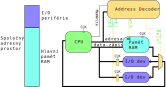
\includegraphics[width=0.8\textwidth]{address_decoder.pdf}
\end{center}
\end{frame}


\begin{frame}
\frametitle{Typy adresových dekodérů}

Centralizovaný dekodér

\begin{center}
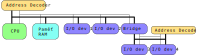
\includegraphics[width=0.8\textwidth]{central.pdf}
\end{center}

Decentralizovaný -- autonomní dekodér

\begin{center}
\includegraphics[width=0.8\textwidth]{distributed.pdf}
\end{center}
\end{frame}

\section{Základní periférie}


\begin{frame}
\frametitle{Asynchronní sběrnice vs. synchronní sběrnice}

Asynchronní sběrnice:
\begin{itemize}
\item  dvě základní varianty:
\begin{itemize}
\item Začátek a konec každého bitu je detekovatelný druhou stranou
\item Je dohodnuta doba trvání vyslání jednoho bitu a jednotlivé bajty mají druhou stranou detekovatelný začátek, případně i konec
\end{itemize}
\item Příkladem asynchronní komunikace je sériový port, USB, SATA disky
\end{itemize}


Synchronní sběrnice:
\begin{itemize}
\item Nejjednodušší je vyhradit jeden signál na přenos hodin vysílajícího k přijímajícímu
\item Vyslání data se řídí hodinami, buď jen jedním typem hrany, nebo i na druhý typ hrany
\item Příkladem synchronního přenosu jsou komunikace DDR s pamětí, PCI, PCI Expres
\end{itemize}
\end{frame}


\begin{frame}
\frametitle{Sériová linka}

\footnotesize
Sériová linka (sériový port) je jedna z nejstarších způsobů komunikace využívaných dodnes.
\begin{itemize}
\footnotesize
\item Asynchronní přenos bez hodin.
\item Obě strany jsou nastaveny na stejnou rychlost, která definuje délku vyslání jednoho bitu
\begin{itemize}
\scriptsize
\item Přenos začíná vysláním start bitu (přechod z 1 $\rightarrow$ 0)
\begin{itemize}
\scriptsize
\item Vysláním a příjmem start bitu se synchronizují lokální hodiny všech zařízení
\end{itemize}
\scriptsize
\item Pak se vysílají jednotlivé bity jednoho bajtu
\item Výběrově pak může následovat bit parity pro kontrolu chyb přenosu
\item Poslední je vyslán stop bit (přechod z 0 $\rightarrow$ 1, nebo přidržení 1)
\end{itemize}
\footnotesize
\item Vyslání jednoho bajtu tedy obsahuje vyslání 10-11 bitů
\item Běžné rychlosti, dříve 9600 Bd až 115200 Bd, nově až 921600 Bd (Bd -- Boud = bit per second)
\end{itemize}

\begin{center}
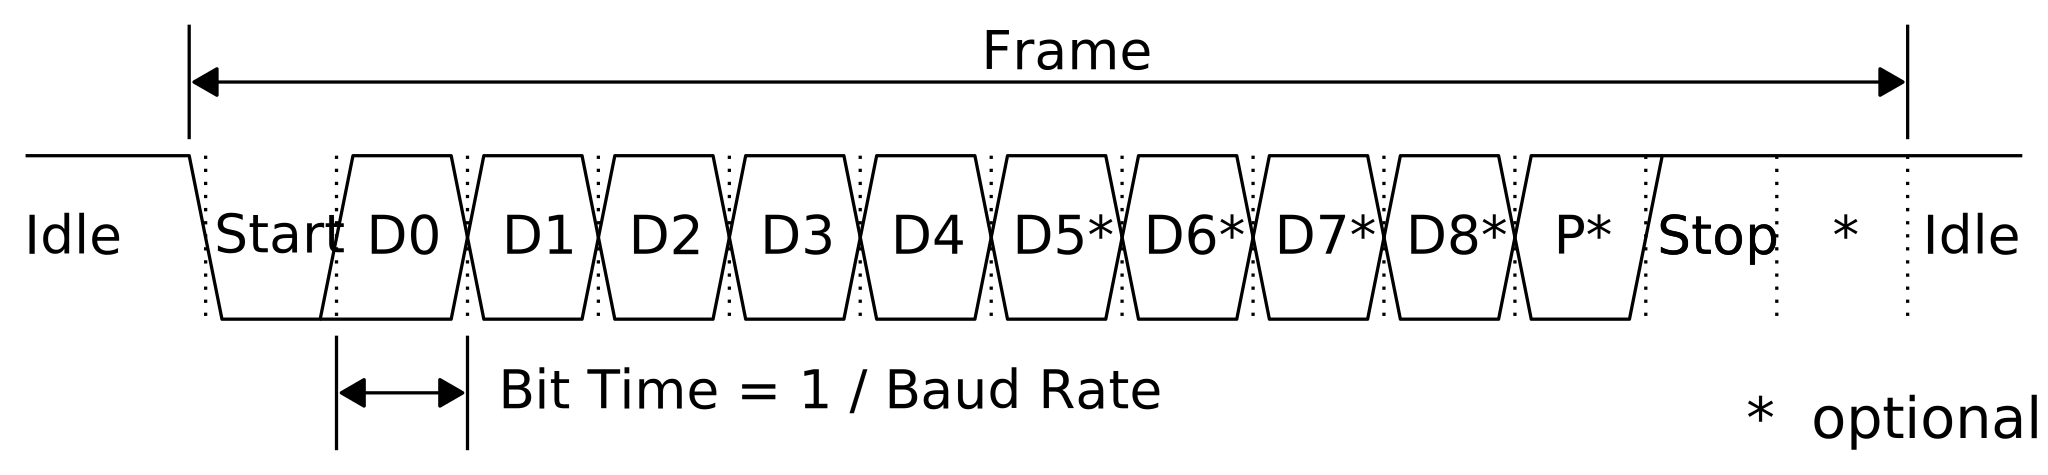
\includegraphics[width=0.8\textwidth]{serial_signals.pdf}
\end{center}
\end{frame}

\begin{frame}[shrink=5]
\frametitle{Sériová linka}

Základní specifikace RS 232:
\begin{itemize}
\item Navrženo pouze pro propojení dvou zařízení
\item Obě zařízení jsou propojené signální zemí
\item 0 reprezentována +3 -- +15V, 1 reprezentuje -3 -- -15 V
\item Plně duplexní, tzn. jiné signály pro přenos tam a jiné pro přenos zpět
\item Mohou být použité signály pro pozdržení vysílání, nebo příjmu při přeplněném lokálním bufferu
\end{itemize}

Základní specifikace RS 422:
\begin{itemize}
\item Plovoucí signál, Rx+, Rx- -- vysílaná hodnota je napětí mezi dvěma vodiči, lze použít až na vzdálenost 1200m
\item Plně duplexní, tzn. jiné signály pro přenos tam a jiné pro přenos zpět
\item Může být více posluchačů pro jednoho vysílajícího
\end{itemize}

Základní specifikace RS 485:
\begin{itemize}
\item Plovoucí signál stejně jako 422
\item Může být half-duplex - tedy pouze dva vodiče, je nutné po vyslání dat odpojit se od sběrnice a poslouchat zda někdo odpoví
\item Lze více zařízení, většinou jeden poveluje, ostatní podle adresy odpovídají
\end{itemize}

\end{frame}

\begin{frame}
\frametitle{UART -- Universal asynchronous receiver-transmiter}

UART -- speciální zařízení, které přijímá a vysílá bajty po sériové lince

\begin{columns}
\begin{column}{0.55\textwidth}  
\begin{itemize}
\item RX\_ST stav přijímání dat
  \begin{itemize}
  \item bit 0 ready -- byla přijata data
  \end{itemize}
\item RX\_DATA přijatá data
  \begin{itemize}
  \item Čtení z adresy RX\_DATA současně odstraní čtená data z UARTu a vymaže příznak ready (pokud nejsou další data)
  \end{itemize}
\item TX\_ST stav odesílání dat
  \begin{itemize}
  \item bit 0 ready -- můžeme zadávat data k odeslání
  \end{itemize}
\item TX\_DATA data k odeslání
  \begin{itemize}
  \item Zápis do TX\_DATA vede rovnou k odesílání data
  \end{itemize}
\end{itemize}
\end{column}
\begin{column}{0.45\textwidth}
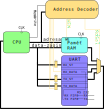
\includegraphics[width=\textwidth]{UART.pdf}
\end{column}
\end{columns}

\end{frame}


\begin{frame}[fragile]
\frametitle{Sériový port v QtRvSim}

\begin{minted}[fontsize=\footnotesize]{gas}
.equ SERIAL_PORT_BASE,   0xffffc000 
#base address of QtRVSim serial port

.equ SERP_RX_ST_REG,       0xffffc000  #Receiver status register
.equ SERP_RX_ST_REG_o,     0x0000      #Offset of RX_ST_REG
.equ SERP_RX_ST_REG_READY_m, 0x1 #Data byte is ready to be read
.equ SERP_RX_ST_REG_IE_m,    0x2 #Enable Rx ready interrupt

.equ SERP_RX_DATA_REG,   0xffffc004 #Received data byte in 8 LSB bits
.equ SERP_RX_DATA_REG_o,   0x0004   #Offset of RX_DATA_REG

.equ SERP_TX_ST_REG,     0xffffc008 #Transmitter status register
.equ SERP_TX_ST_REG_o,     0x0008   #Offset of TX_ST_REG
.equ SERP_TX_ST_REG_READY_m,  0x1 #Transmitter can accept next byte
.equ SERP_TX_ST_REG_IE_m,     0x2 #Enable Tx ready interrupt

.equ SERP_TX_DATA_REG,   0xffffc00c #Write word to send 8 LSB bits
.equ SERP_TX_DATA_REG_o,   0x000c   #Offset of TX_DATA_REG
\end{minted}
\end{frame}

\begin{frame}[fragile]
\frametitle{Příklad vyslání znaku}

\begin{minted}[fontsize=\footnotesize]{gas}
write:
    li   a0, SERIAL_PORT_BASE # a0 ukazuje na zacatek pameti UART
    la   a1, text_1           # nacti ukazatel na retezec
next_char:
    lb   t1, 0(a1)            # nacti znak k odeslani
    beq  t1, zero, end_char   # 0 ukoncuje retezec
    addi a1, a1, 1            # posun ukazatel
tx_busy:
    lw   t0, SERP_TX_ST_REG_o(a0)       # zjisti statu odesilaci fronty
    andi t0, t0, SERP_TX_ST_REG_READY_m # vymaskuj bit READY
    beq  t0, zero, tx_busy    # pokud neni volno v UARTU cekej zkus to znovu
    sw   t1, SERP_TX_DATA_REG_o(a0) # je volno - zapis bajt
    j    next_char            # posli dalsi znak
end_char:
    ebreak                    # ukonci program

    .data
text_1:
    .asciz  "Hello world.\n"  # retezec ukonceny 0
\end{minted}

\end{frame}

\begin{frame}[fragile]
\frametitle{Příklad přijetí znaku}

\begin{minted}[fontsize=\footnotesize]{gas}
gets: li   a0, SERIAL_PORT_BASE # a0 ukazuje na zacatek pameti UART
    la   a1, text_1           # nacti ukazatel na buffer
    addi t2, zero, 40
next_char:
rx_not_ready:
    lw   t0, SERP_RX_ST_REG_o(a0)       # zjisti statu prijimaci fronty
    andi t0, t0, SERP_RX_ST_REG_READY_m # vymaskuj bit READY
    beq  t0, zero, rx_not_ready    # pokud neni znak UARTU cekej zkus to znovu
    lw   t1, SERP_RX_DATA_REG_o(a0) # je znak - precti ho a tim odstran
    sb   t1, 0(a1)            # uloz znak do bufferu
    addi t1, t1, -13          # test je to novy radek?
    beq  t1, zero, end_char   # ukoncuje cteni
    addi a1, a1, 1            # posun ukazatel
    addi t2, t2, -1            # kontroluj kolik muzeme nacist
    bne  t2, zero, next_char
end_char:
    ebreak                    # ukonci program
    .data
text_1:
    .word 0,0,0,0,0,0,0,0,0,0
\end{minted}
\end{frame}



\begin{frame}
\frametitle{QtRvSim Terminal -- serial port}
\begin{center}
\includegraphics[width=0.8\textwidth]{fig/QtRvSim-serial-normal.png}
\end{center}
\end{frame}

\begin{frame}
\frametitle{QtRvSim Terminal -- serial port}
\begin{center}
Zřetězený procesor -- pipelined verze
\includegraphics[width=0.8\textwidth]{fig/QtRvSim-serial-normal.png}
\end{center}
\end{frame}

\begin{frame}
\frametitle{Shrnutí komunikace periferií}

\begin{itemize}
\item uvedený způsob komunikace je tzv. pooling
\begin{itemize}
\item program se neustále dotazuje, zda se něco nezměnilo, nepřišel znak, nebo se uvolnila odesílací fronta
\item toto je velmi neefektivní, zatěžuje zbytečně CPU, které by mohlo dělat něco užitečného
\end{itemize}
\item na přednášce 9 bude využití přerušení
\begin{itemize}
\item program může dělat něco jiného, přerušení nastane, pokud je povoleno a změní se stav periférie
\item při přerušení se začne provádět jiný program, který zjistí, jaká událost se stala a zpracuje ji
\item informace o tom co se stalo předá programu pomocí synchronizačních prostředků (bude v podrobně v předmětu OSY)
\end{itemize}
\end{itemize}

\end{frame}


\begin{frame}[fragile]
\frametitle{QtRvSim -- otočné voliče, led}

\begin{columns}
\begin{column}{0.6\textwidth}  
\begin{minted}[fontsize=\footnotesize]{gas}
#base of SPILED port region
.equ SPILED_REG_BASE,       0xffffc100

#RGB LED 1 barevne slozky – 8 bitu kazda
.equ SPILED_REG_LED_RGB1,   0xffffc110
.equ SPILED_REG_LED_RGB1_o,   0x0010

#RGB LED 2 barevne slozky – 8 bitu kazda
.equ SPILED_REG_LED_RGB2,   0xffffc114
.equ SPILED_REG_LED_RGB2_o,   0x0014

#Tri 8 bitove otocne volice
#nejvyssi bajt informace o stitsknuti
.equ SPILED_REG_KNOBS_8BIT, 0xffffc124 
.equ SPILED_REG_KNOBS_8BIT_o, 0x0024

#32 LEDek kazdy bit jedna LED dioda
.equ SPILED_REG_LED_LINE,   0xffffc104
.equ SPILED_REG_LED_LINE_o,   0x0004
\end{minted}
\end{column}
\begin{column}{0.4\textwidth}
\includegraphics[width=\textwidth]{fig/knobs.png}
\end{column}
\end{columns}

\end{frame}

\begin{frame}[fragile]
\frametitle{Příklad použití informace od otočných voličů}

\begin{minted}[fontsize=\footnotesize]{gas}
    li   a0, SPILED_REG_BASE # a0 ukazuje na zacatek pameti pro I/O
    ori  t2, t2, -1
loop:
    lw   t0, SPILED_REG_KNOBS_8BIT_o(a0)   # nacti data od otocnych volicu
    sw   t0, SPILED_REG_LED_RGB1_o(a0)
    xor  t1, t0, t2
    sw   t1, SPILED_REG_LED_RGB2_o(a0)
    srli t0, t0, 24
    andi t0, t0, 4
    beq  t0, zero, loop    # pokud nebyl zmacknut cerveny volic

    ebreak                    # ukonci program
\end{minted}
\end{frame}

\section{Sběrnice}

\begin{frame}
\frametitle{Co je sběrnice?}

\end{frame}

\begin{frame}
\frametitle{Topologie sběrnic}

\end{frame}

\begin{frame}
\frametitle{PC sběrnice}
Stará architktura

Severní můstek, Jižní můstek, bridge
\end{frame}

\begin{frame}
\frametitle{PC sběrnice}

Moderní s ovladačem paměti na čipu.
\end{frame}

\begin{frame}
\frametitle{PCI}

Jak funguje PCI
\end{frame}

\begin{frame}
\frametitle{Signály a přenos dat}

\end{frame}

\begin{frame}
\frametitle{PCI architektura}

\end{frame}

\begin{frame}
\frametitle{Přenos adresy a přenos dat}

\end{frame}

\begin{frame}
\frametitle{Čtení dat z periférie}

\end{frame}

\begin{frame}
\frametitle{PCI Expres -- PCIe}

Výhody sériového rozhraní oproti čistě paralelnímu

\end{frame}

\begin{frame}
\frametitle{Ukázka omezení rychlosti pro paralelní}

\end{frame}


\begin{frame}
\frametitle{PCIe rychlosti a přenosové kapacity}

\end{frame}

\begin{frame}
\frametitle{PCIe x1-x16}

\end{frame}



\begin{frame}
\frametitle{PCIe topologie}

\end{frame}

\begin{frame}
\frametitle{Realita signálů sériové sběrnice}

Vzhled signálů v závisloti na vzdálenosti.

\end{frame}


\begin{frame}
\frametitle{Hard disky}

Od ATA PATA k SATA
asi více slajdů
\end{frame}


\end{document}

